\documentclass[12pt,aspectratio=169]{beamer}
\usepackage[utf8]{inputenc}
\usepackage[T1]{fontenc}
\usepackage{lmodern}
\usepackage[english]{babel}
\usepackage{hyperref}
\usetheme{metropolis}
\begin{document}
	\author{Benjamin William Kaufold}
	\title{{\huge OpenMolcas: Labeling Specific Orbitals for Inclusion in MR Active Space}}
	%\subtitle{}
	%\logo{}
	\institute{Northeastern University}
	%\date{}
	%\subject{}
	%\setbeamercovered{transparent}
	%\setbeamertemplate{navigation symbols}{}
	\begin{frame}[plain]
		\maketitle
	\end{frame}

	\begin{frame}{Summary}
		\begin{columns}
			\begin{column}{.5\linewidth}
				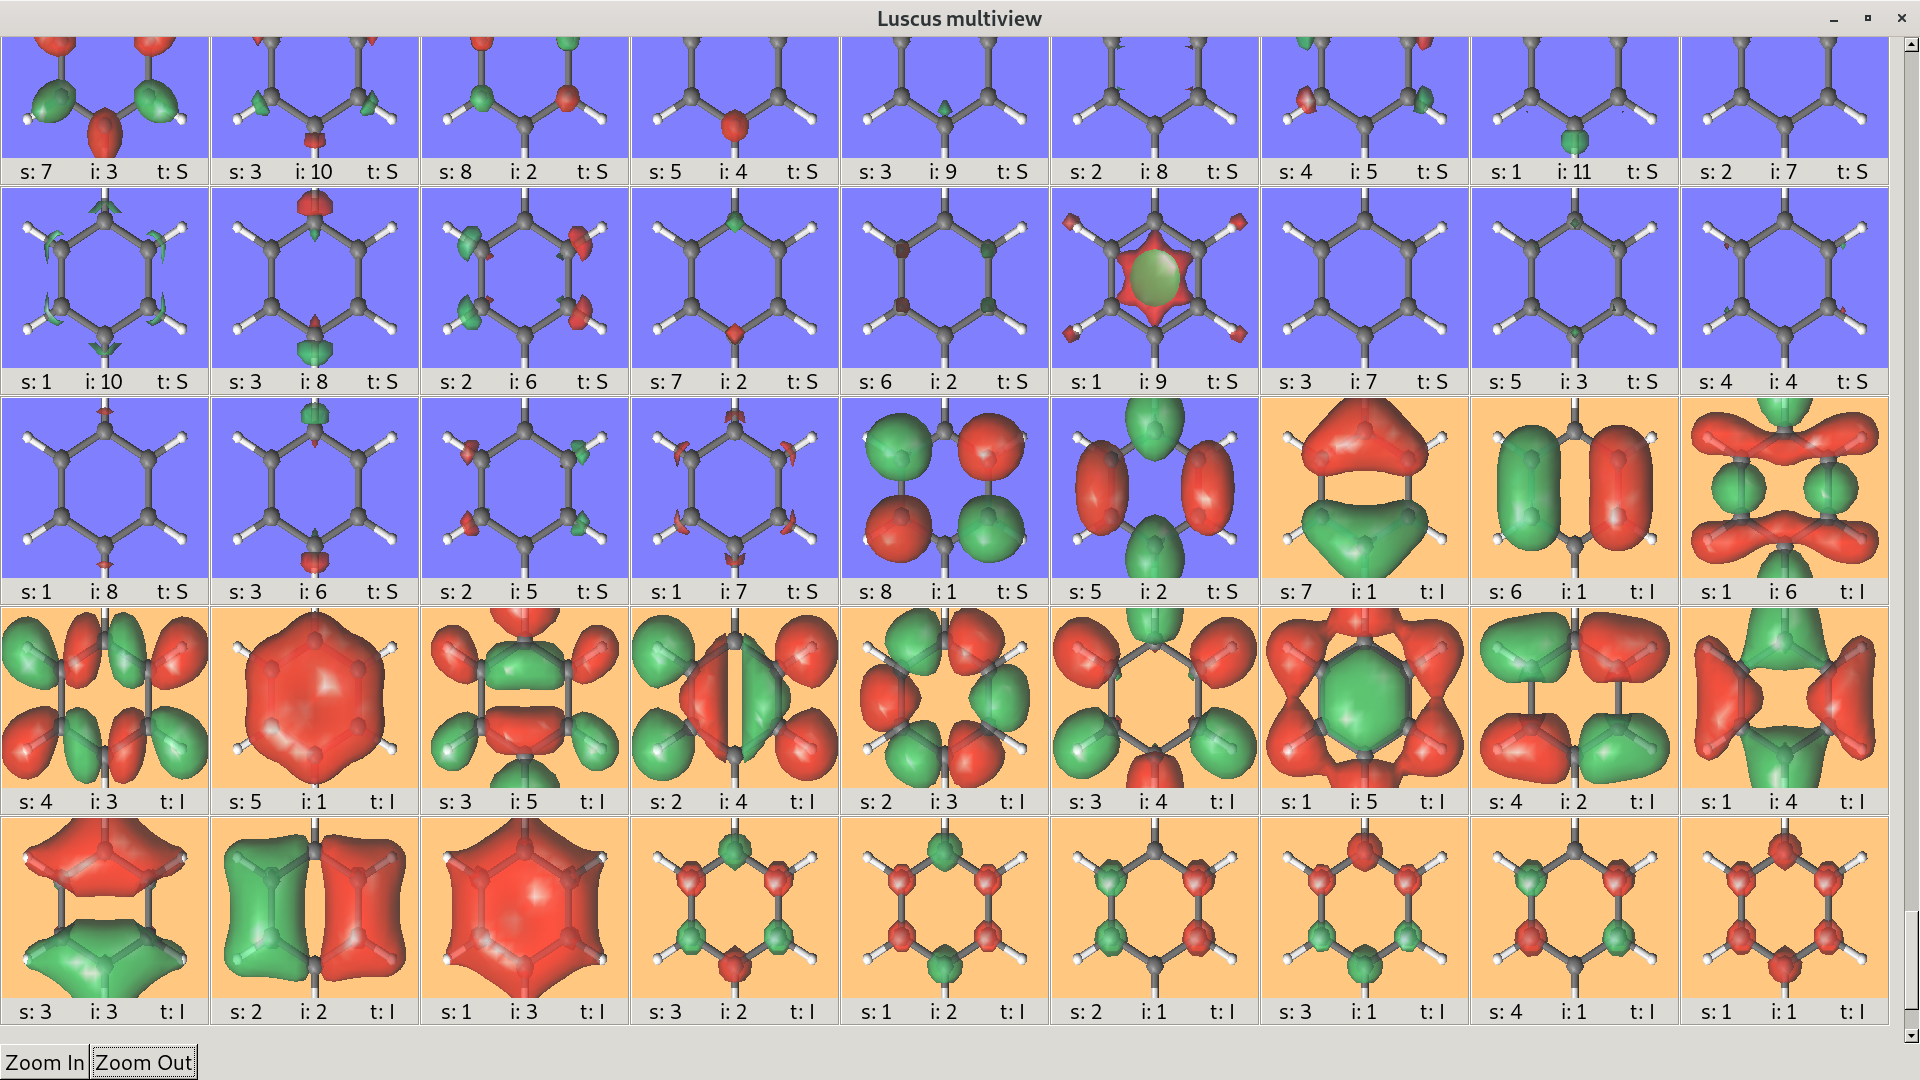
\includegraphics[width=\linewidth]{all.png}
			\end{column}
			\begin{column}{.5\linewidth}
				It is possible to flag specific orbitals for inclusion in the active space for multireference calculations in OpenMolcas.  The method presented in the workshop offers finer control than simply specifying the number of active electrons and orbitals and does not require the use of symmetry (but is compatible with it).
			\end{column}
		\end{columns}
	\end{frame}

	\begin{frame}{Potential Benefits and Caveats}
		\begin{itemize}
			\item Useful if one wants to study an excitation with a specific character, e.g. to compare to literature
			\item Allows for smaller active spaces to capture excitations that normally require large active spaces
			\item Can be used to determine the importance of specific orbitals for describing a system
			\item Eschews the use of the "Alter" keyword and does not require a test CASSCF calculation, only a preceding SCF
			\item \textbf{Is not guaranteed to make calculations more accurate} (and isn't meant to); just gives users more options
			\item \textbf{Is not useful for mass/automated calculations} since the user must visualize and choose the desired orbitals
		\end{itemize}
	\end{frame}

	\begin{frame}[fragile]{Basic Procedure}
		\begin{columns}
			\begin{column}{.25\linewidth}
				\begin{scriptsize}
					\begin{verbatim}
						#INDEX
						* 1234567890
						0 iiiiiiiiii
						1 iiiiii2ii2
						2 222sssssss
						3 ssssssssss
						4 ssss2sssss
						5 ssssssssss
						6 ssssssssss
						7 ssssssssss
						8 ssssssssss
						9 ssssssssss
						0 ssssssssss
						1 ssssssssss
						2 ssssssssss
						3 ssssssssss
						4 ssssssssss
						5 ssssssssss
						...
					\end{verbatim}
				\end{scriptsize}
			\end{column}
			\begin{column}{.75\linewidth}
				%\begin{footnotesize}
					\begin{enumerate}
					\item Generate starting orbitals in OpenMolcas using the SCF module as normal, making sure to produce a Luscus file as well
					\item Create a copy of the .ScfOrb file produced by Step 1
					\item View the orbitals in Luscus and determine the indices of the orbitals to include in the active space
					\item At the very bottom of the new .ScfOrb file from Step 2, replace ``i'' or ``s'' with ``2'' for orbitals that should be included in the active space
					\item Run a CASSCF calculation, using the keyword FileOrb to use your custom active space; specify nActEl but not Ras2
				\end{enumerate}
				%\end{footnotesize}
			\end{column}
		\end{columns}
	\end{frame}

	\begin{frame}{Detailed Procedure}
		\begin{columns}
			\begin{column}{.5\linewidth}
				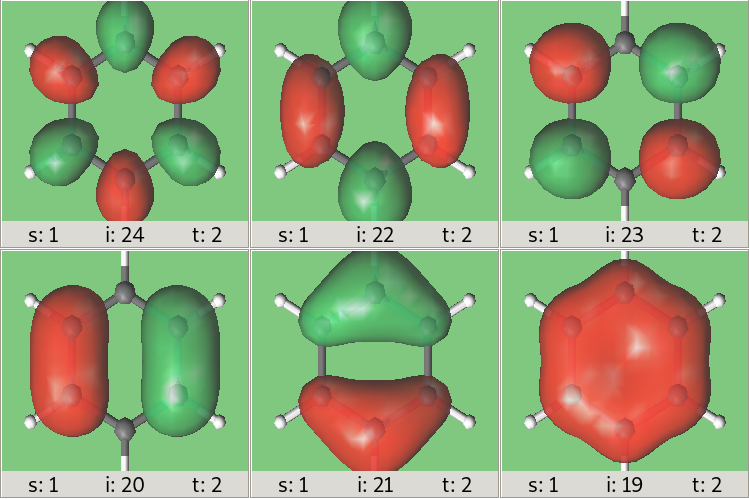
\includegraphics[width=\linewidth]{manual.png}
			\end{column}
			\begin{column}{.5\linewidth}
				\begin{footnotesize}
					
					
					The benzene molecule has a simple ``intuitive'' active space consisting of all valence $\pi$ system orbitals.  This set obeys the correlating orbital principle, and moreover, $\pi$-type orbitals are considered useful in active spaces (while $\sigma$-type orbitals are usually not except when lone pairs or strain are involved).  The example shown will force OpenMolcas to use these orbitals in a set of MR[6,6] calculations without taking advantage of symmetry.  
					
					The starting geometry was optimized with B3LYP/aug-cc-pVTZ in Gaussian.  Assume all files are in the same folder.
					
					
				\end{footnotesize}
			\end{column}
		\end{columns}
	\end{frame}

	\begin{frame}[fragile]{Starting Structure (optimized.xyz)}
		\begin{footnotesize}
			\begin{verbatim}
			12
			
			H         0.000000000000      2.472664049111      0.000000000000
			H         2.141703184311      1.235977868265      0.000000000000
			C         0.000000000000      1.390832830975      0.000000000000
			H        -2.141703184311      1.235977868265      0.000000000000
			C         1.204662535154      0.695342547527      0.000000000000
			C        -1.204662535154      0.695342547528      0.000000000000
			C         1.204662535154     -0.695342547528      0.000000000000
			C        -1.204662535154     -0.695342547527      0.000000000000
			H         2.141703184311     -1.235977868265      0.000000000000
			C         0.000000000000     -1.390832830975      0.000000000000
			H        -2.141703184311     -1.235977868265      0.000000000000
			H         0.000000000000     -2.472664049111      0.000000000000
		\end{verbatim}
		\end{footnotesize}
	\end{frame}

	\begin{frame}[fragile]{OpenMolcas Input for Orbital Generation (orbitals-C1.inp)}
		\begin{columns}
			\begin{column}{.5\linewidth}
				\begin{scriptsize}
			\begin{verbatim}
			&GATEWAY
			Title = Benzene Orbitals with Symmetry
			Coord = optimized.xyz
			Basis = aug-cc-pVTZ
			Group = NoSym
			
			&SEWARD
			grid input
			grid=ultrafine
			end of grid input
			
			&SCF
			KSDFT = B3LYP
			
			&GRID_IT
			Sparse; Pack
			All
		\end{verbatim}
		\end{scriptsize}
			\end{column}
			\begin{column}{.5\linewidth}
				\begin{itemize}
					\item Ultrafine grid used in \&SEWARD to generate more accurate starting orbitals for MR (recommended by OpenMolcas)
					\item ``Sparse, Pack'' keywords in \&GRID\_IT reduce the size of the Luscus file without affecting the orbitals in .ScfOrb; usually still good enough for visualization (but not for printing)
				\end{itemize}
			\end{column}
		\end{columns}
	\end{frame}

	\begin{frame}{Analyzing Orbitals (orbitals-C1.lus)}
		\begin{columns}
			\begin{column}{.5\linewidth}
				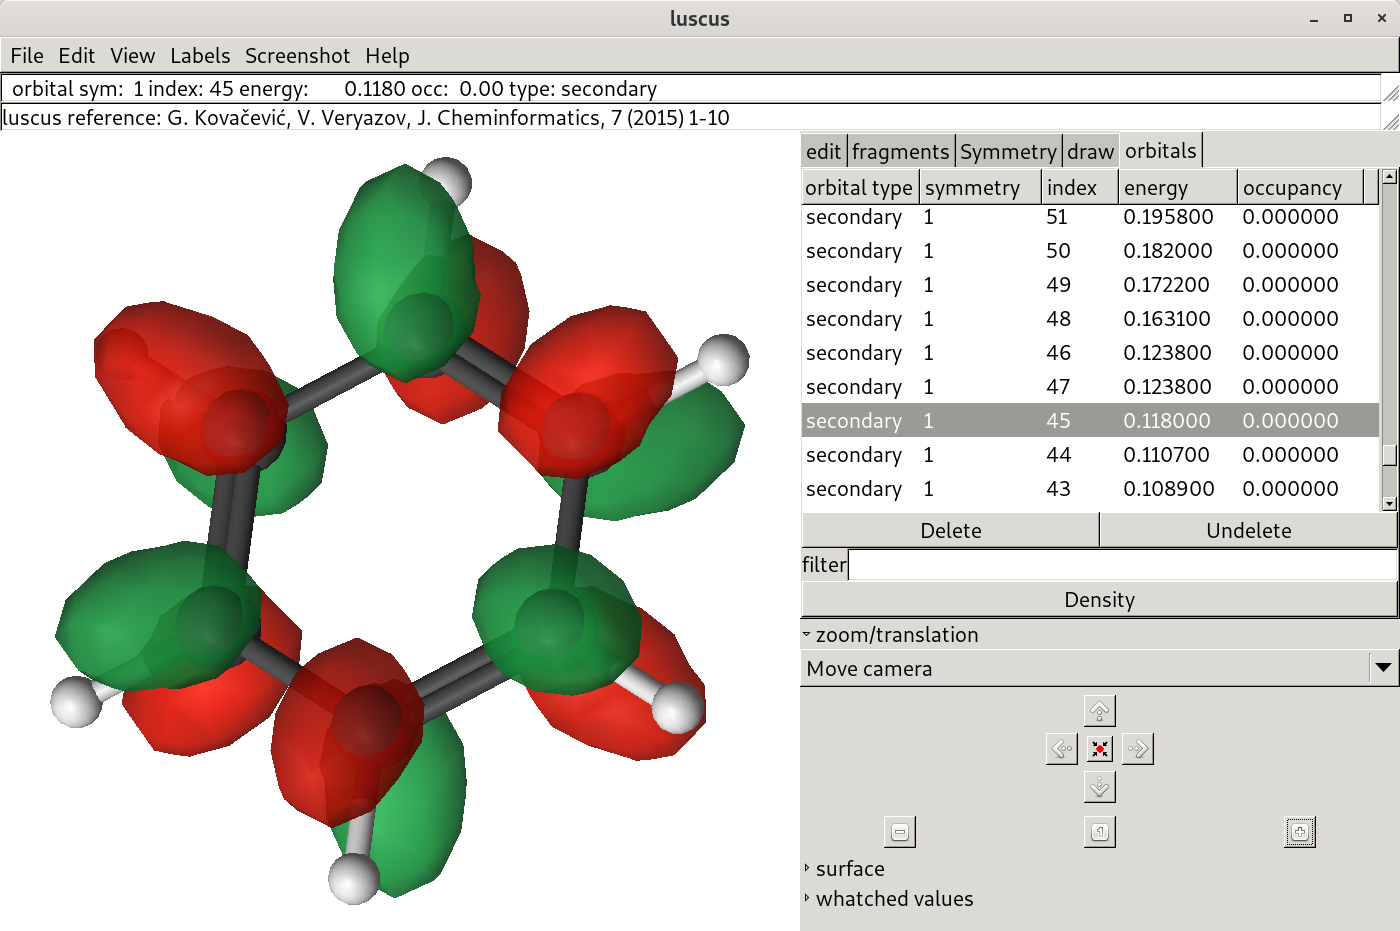
\includegraphics[width=\linewidth]{analyze.png}
			\end{column}
			\begin{column}{.5\linewidth}
				The orbitals belonging to the $\pi$ system are:
				
				17, 20, 21, 22, 23, 45
				
				17, 20 and 21 have label ``i'' meaning fully occupied; 22, 23 and 45 have label ``s'' meaning empty.  There is an empty correlating orbital for every occupied valence orbital.
			\end{column}
		\end{columns}
	\end{frame}

	\begin{frame}[fragile]{Labeling Orbitals for Active Space (Copy of orbitals-C1.ScfOrb)}
		\begin{columns}
			\begin{column}{.5\linewidth}
				
				
				Before Editing
				\begin{verbatim}
					#INDEX
					* 1234567890
					0 iiiiiiiiii
					1 iiiiiiiiii
					2 isssssssss
					3 ssssssssss
					4 ssssssssss
					5 ssssssssss
					...
				\end{verbatim}
			\end{column}
			\begin{column}{.5\linewidth}
				
				
				After Editing
				\begin{verbatim}
					#INDEX
					* 1234567890
					0 iiiiiiiiii
					1 iiiiii2ii2
					2 222sssssss
					3 ssssssssss
					4 ssss2sssss
					5 ssssssssss
					...
				\end{verbatim}
			\end{column}
		\end{columns}
		The orbital label is 10 times the row label plus the column label.
	\end{frame}

	\begin{frame}[fragile]{Multireference Calculation (mr-C1.inp)}
		\begin{columns}
			\begin{column}{.5\linewidth}
				\begin{scriptsize}
					\begin{verbatim}
					&GATEWAY
					Title = Benzene MR with Symmetry
					Coord = optimized.xyz
					Basis = aug-cc-pVTZ
					Group = NoSym
					
					&SEWARD
					grid input
					grid=ultrafine
					end of grid input
					
					&RASSCF
					FileOrb = labeled-C1.ScfOrb
					nActEl = 6
					Charge = 0
					Spin = 1
					CIRoot = 6 6 1
					OutOrbital = Natural; 6
					
					...
				\end{verbatim}
				\end{scriptsize}
			\end{column}
			\begin{column}{.5\linewidth}
				\begin{itemize}
					\item In \&RASSCF, use FileOrb = " to give the name of your manually flagged SCF orbitals
					\item Still specify the number of active electrons, not no need to specify the number of active orbitals
					\item No need to make changes to any of the following modules, e.g. \&CASPT2 and \&MCPDFT; the active space is ``decided'' in the \&RASSCF module
				\end{itemize}
			\end{column}
		\end{columns}
	\end{frame}
	\begin{frame}{Differences in Active Spaces}
		\begin{columns}
			\begin{column}{.5\linewidth}
				
				
				Manually Chosen Active Space
				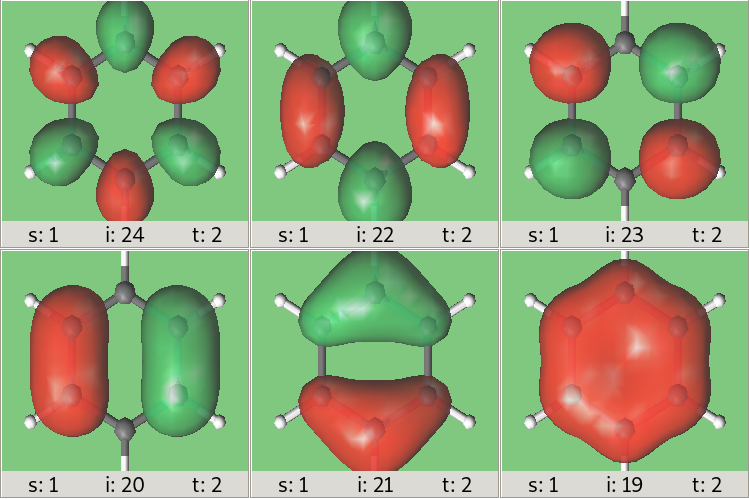
\includegraphics[width=\linewidth]{manual.png}
			\end{column}
			\begin{column}{.5\linewidth}
				
				
				Automatic [6,6] Active Space
				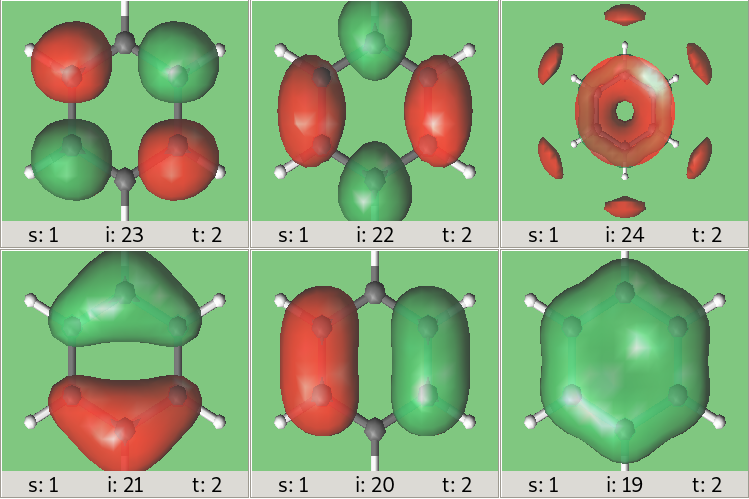
\includegraphics[width=\linewidth]{automatic.png}
			\end{column}
		\end{columns}
		When the active space is not manually chosen, the completely in-phase $\pi$ orbital does not have a correlating orbital; instead a $\sigma$-type Rydberg orbital is chosen (altered zoom and isovalue for clarity).
	\end{frame}

	{
		\setbeamertemplate{footline}{Micka\"{e}l V\'{e}ril \textit{et. al.}, ``QUESTDB: A database of highly accurate excitationenergies for the electronic structure community'', WIREs Comput Mol Sci.2021;11:e1517}
	\begin{frame}{Excitation Energies (eV)}
		\begin{center}
			\begin{tabular}{|c|c|c|c|c|c|}
				\hline
				Calculation & S\textsubscript{1} & S\textsubscript{2} & S\textsubscript{3} & S\textsubscript{4} & S\textsubscript{5} \\
				\hline
				CASPT2[6,6]/aug-cc-pVTZ (Manual) & 5.19 & 5.88 & 6.15 & 8.12 & 8.14 \\
				CASPT2[6,6]/aug-cc-pVTZ (Automatic) & 4.72 & 6.21 & 6.78 & 6.78 & 9.84 \\
				\hline
			\end{tabular}
			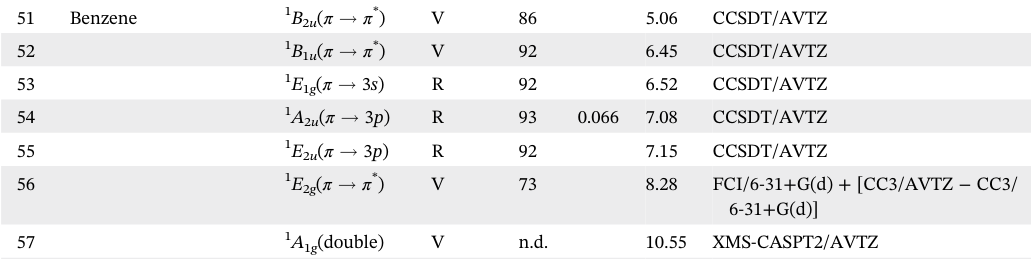
\includegraphics[width=.9\linewidth]{quest.png}
		\end{center}
		\begin{small}
			Manually choosing the active space allows us to capture certain excitations that cannot normally be accessed with [6,6] such as $^1E_{2g}(\pi\rightarrow\pi^*)$.  But low-lying excitation energies are not necessarily more accurate.
		\end{small}
	\end{frame}
	}
	\begin{frame}{Note: A Graphical Alternative}
		\begin{columns}
			\begin{column}{.5\linewidth}
				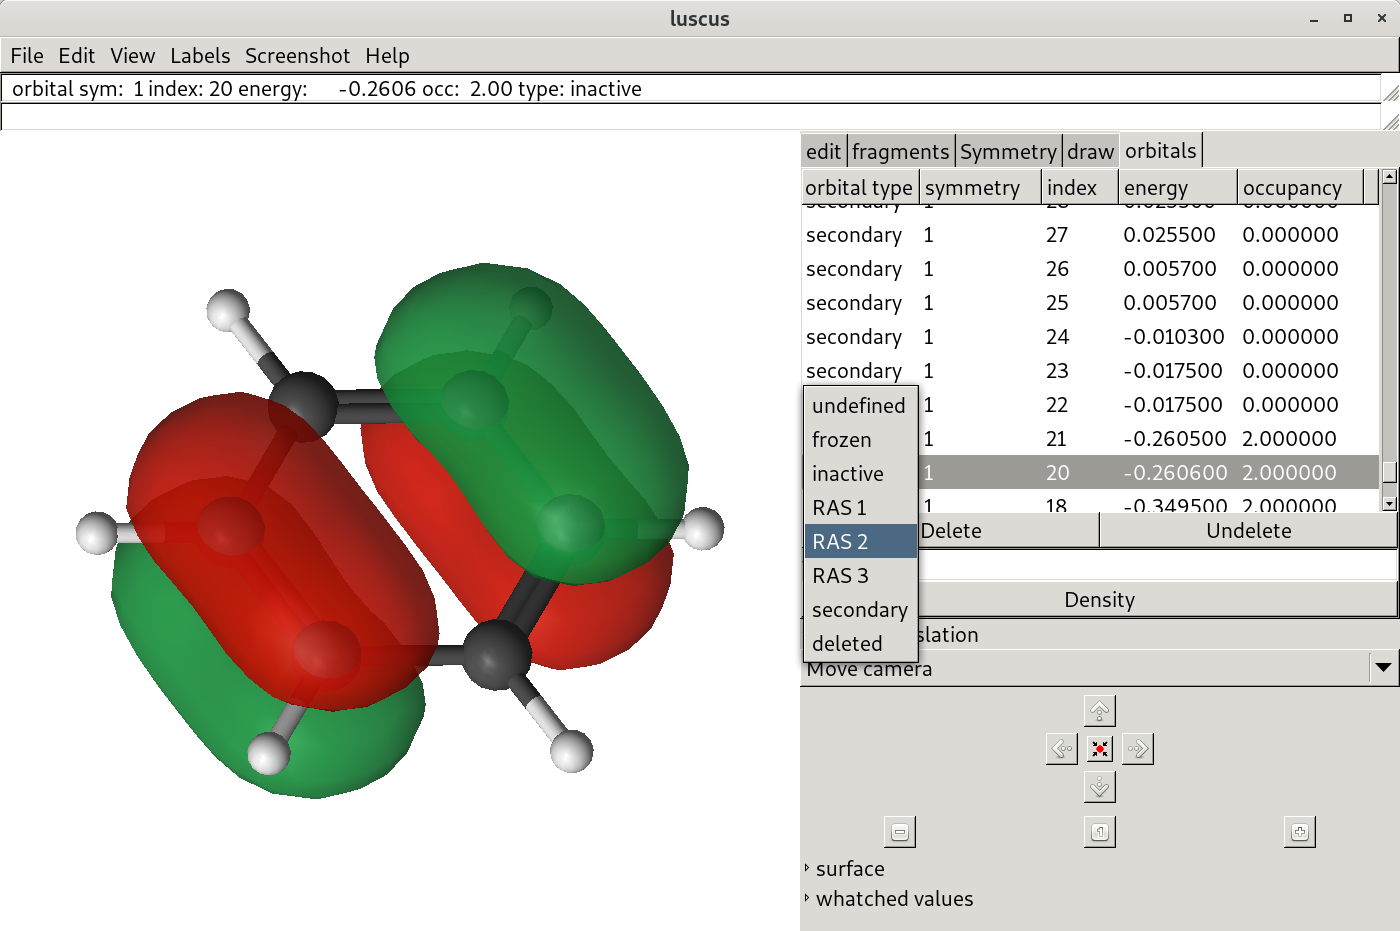
\includegraphics[width=\linewidth]{select.png}
			\end{column}
			\begin{column}{.5\linewidth}
				
				
				Luscus can also be used to select the active space without the need to manually edit the text file.
				\begin{enumerate}
					\item Open the Luscus file for the SCF calculation
					\item Use a drop-down to change the orbital type to RAS2 as desired
					\item File > Save As... a .GvOrb file in a known location
					\item Use this as your starting orbitals in \&RASSCF with FileOrb = "
				\end{enumerate}
			\end{column}
		\end{columns}
	\end{frame}

	\begin{frame}{Additional Notes}
		\begin{itemize}
			\item Make sure the orbitals you choose is consistent with the number of electrons (i.e. for a [6,6] calculation, choose three occupied and three empty orbitals)
			\begin{itemize}
				\item OpenMolcas will automatically adjust the active space otherwise
			\end{itemize}
			\item If your calculation uses symmetry, there will be multiple tables with ``i'' and ``s'' labels for orbitals, in order of symmetry index; edit them separately
			\begin{itemize}
				\item For complicated cases it is probably easier to just use Luscus to do this
			\end{itemize}
			\item Orbitals may change during the optimization procedure if the choice of active space is completely unreasonable (core orbitals, broken degeneracy, etc.)
			\begin{itemize}
				\item Always check afterwards that the orbitals you wanted to include in the active space are actually there!
			\end{itemize}
		\end{itemize}
	\end{frame}

	
\end{document}